\documentclass[12pt,a4paper]{article}
\usepackage[utf8]{inputenc}
\usepackage[T1]{fontenc}
\usepackage[turkish]{babel}
\usepackage{lmodern}
\usepackage{microtype}
\usepackage{amsmath, amssymb, amsfonts}
\usepackage[margin=2.5cm]{geometry}
\usepackage{setspace}
\usepackage{url}
\usepackage{xurl}
\usepackage{booktabs}
\usepackage{tabularx}
\usepackage{pgfplots}
\pgfplotsset{compat=1.18}
\usetikzlibrary{babel}

\onehalfspacing

\title{\textbf{Grand Proof II: Navier--Stokes Girdap Doyumundan 4B SU(3) Yang--Mills Kütle Aralığına İzomorfizm ve Lattice QCD Glueball Spektrumu} \\[0.3cm]
\large (Kuark Kuşatması ve Charmonium/Bottomonium Yarılmaları, Sıfır Serbest Parametre)}
\author{Fahri Meral}
\date{19 Ekim 2026}

\begin{document}
\shorthandoff{=}

\maketitle

\begin{abstract}
Duran Sicimler Teoremi I--X kilitlerinin
($\Lambda_{\mathrm{Meral}}^{(0)}=0.0722694327$;
$\mu_s^{\mathrm{Meral}}=0.2044088237$; $\beta_0=1/2$;
$\eta_{\mathcal{T}_0}=0.1434$; $\mathcal{C}_{\mathrm{univ}}=1.626038$)
kapalı gluon akı halkası kuantizasyonuna taşınmasıyla Clay Milenyum problemi
Yang--Mills kütle aralığına sıfır-parametreli köprü kurulmaktadır:
\begin{enumerate}
    \item \textbf{Akı-Tüpü Operatörü (Teorem GP-II.1, Test T32):}
    Tekilliksiz etkin potansiyel
    $V_{\mathrm{eff}}(x)=(1+\beta_0^2)/(x^2+\beta_0^2)
    +\mathcal{C}_{\mathrm{univ}}^2(1+\mu_s^{\mathrm{Meral}})x^2$
    altında $\mathcal{H}_{\mathrm{YM}}$ kesin pozitiftir
    ($\lambda_0=5.9158<\lambda_1<\lambda_2$,
    $|\langle u_0|u_1\rangle|<10^{-14}$); OS transfer korelasyonu
    $G_c(t)>0$ olup iki-noktalı eğimi radyal aralığa
    $\lambda_1-\lambda_0=6.6237$ yakınsar; Richardson süreklilik limiti
    sonludur ($\lambda_0^{\mathrm{cont}}\approx 5.77$, ölçülen mertebe
    $p\approx 0.28$). Kapalı-form aralık
    $\Delta m_{\mathrm{gap}}/\sqrt{\sigma}=3.3914463$,
    Lattice QCD $3.405\pm 0.021$ ile \%0.40 fark ($0.65\,\sigma$) verir.
    \item \textbf{Glueball Spektrumu (Teorem GP-II.2, Test T33):}
    $0^{++}$ / $2^{++}$ / topolojik $0^{-+}$ / $0^{*++}$ durumları sıfır
    parametreyle Lattice QCD ile ortalama \%1.56 farkla uyuşur
    (topolojisiz klasik $0^{-+}=4.8803$ karşılaştırma için korunur).
    \item \textbf{Kuark Kuşatması (Teorem GP-II.3/3b, Test T34):}
    $\gamma_{\mathrm{Meral}}=\frac{\pi}{12}(1+\frac{4}{5}\kappa_{\mathrm{Meral}})$
    $=0.29847153$, Cornell katsayısı $0.295\pm 0.010$ ile \%1.18
    ($0.35\,\sigma$) örtüşür; charmonium $2S$--$1S$ saf-IR'de $581.03$ MeV
    (PDG $589.19$, \%1.39) bulunur. Sıfır-parametreli UV--IR varyantı
    bottomoniumu $456.43$ MeV'den $645.80$ MeV'ye taşır (PDG $562.96$;
    işaret değiştirir, \%14.7) ancak charmoniumu bozar; birincil sonuç
    saf-IR kalır (detay Bölüm 5).
\end{enumerate}
Sayısal doğrulama zinciri \texttt{T1--T34 (34/34 PASS)} ve bağımsız çapraz kontrol
betiği (\path{mini_check_gp2.py}, \texttt{15/15 PASS}) tam geçer.
\end{abstract}

\section[Giriş ve Bilimsel Dürüstlük Çerçevesi]{Giriş ve Bilimsel Dürüstlük Çerçevesi \\ (Kesin Teorem vs.\ Lattice Verisi vs.\ İzomorfizm Köprüsü)}

Clay Milenyum problemlerinden Yang--Mills kütle aralığı [1] şunu sorar: klasik
Lagrange yoğunluğunda kütlesiz gluonlar neden uzun mesafede serbest kalamaz ve
en düşük vakum-üstü uyarılma (skaler glueball $0^{++}$) neden kesin pozitif
kütleye sahiptir? Navier--Stokes girdap iplikçikleri ile $SU(3)$ kromoelektrik
akı tüpleri aynı silindirik eksenel geometriyi paylaşır: Teorem 2 eksen
düzenlemesi ($\beta_0=1/2$) ve Teorem 5 FENE-P doyumu tekilliği kaldırır;
Teorem 9 Hessian pozitivliği koersif kuyu verir ve koersif kuyunun taban enerjisi
sıfırdan kesin büyüktür.

\textbf{Üç katmanlı dürüstlük ayrımı:}
\begin{itemize}
    \item \textbf{Kesin Matematiksel Teorem:} Tekilliksiz radyal operatör
    (Denk.~\ref{eq:veff}), koersiflik ve $\lambda_0>0$ (Denk.~\ref{eq:gap}),
    Cornell bağlı-durum özdeğerleri --- sıfır serbest parametre.
    \item \textbf{Bağımsız literatür (model dışı):} Lattice QCD glueball
    oranları [2--4], Lüscher sabiti $\pi/12$ [5], Cornell katsayısı [6,7],
    PDG kuarkonyum yarılmaları [8].
    \item \textbf{İzomorfizm köprüsü (sınamaya açık):} Kilitli I--X
    sabitlerinin halka kuantizasyonuna taşınması; spin-bağımsız statik
    potansiyel ansatzı.
\end{itemize}
Kilitli girdiler: $\Lambda_{\mathrm{Meral}}^{(0)} = 0.07226943267767906$,
$\mu_s^{\mathrm{Meral}} = 0.2044088237$, $\beta_0 = 1/2$,
$\eta_{\mathcal{T}_0} = 0.1434$,
$\mathcal{C}_{\mathrm{univ}} = 1.626038$. Yeni kalibrasyon parametresi yoktur.

\section{Görev 26 / Test T32 --- Akı-Tüpü Operatörü ve Kütle Aralığı}

Boyutsuz kesit koordinatı $x=r\sqrt{\sigma}$ üzerinde etkin Hamiltonyen
$\mathcal{H}_{\mathrm{YM}}=-\frac{1}{x}\partial_x(x\partial_x)+V_{\mathrm{eff}}$
olsun. İnce-sicim modelindeki $-(\pi/12)/x^2$ tekilliğine karşı:

\textbf{Teorem GP-II.1 (Tekilliksiz Akı-Tüpü ve Kesin Pozitif Aralık):}
\textit{$\beta_0=1/2$, $\mu_s^{\mathrm{Meral}}>0$ altında etkin potansiyel}
\begin{equation}
\label{eq:veff}
\boxed{V_{\mathrm{eff}}(x)=\frac{1+\beta_0^2}{x^2+\beta_0^2}
+\mathcal{C}_{\mathrm{univ}}^2(1+\mu_s^{\mathrm{Meral}})\,x^2}
\end{equation}
\textit{her $x\ge 0$ için pozitiftir ($V_{\min}=3.19416$); $\mathcal{H}_{\mathrm{YM}}$
kendine-eşlenik Sturm--Liouville operatörü olup
$\lambda_0=\inf\langle\psi,\mathcal{H}_{\mathrm{YM}}\psi\rangle>0$ kesin
pozitiftir. Kapalı halka kuantizasyonu:}
\begin{equation}
\label{eq:gap}
\boxed{\frac{\Delta m_{\mathrm{gap}}^{\mathrm{Meral}}(0^{++})}{\sqrt{\sigma}}
=2\,\mathcal{C}_{\mathrm{univ}}\sqrt{1+\tfrac{1}{2}\mu_s^{\mathrm{Meral}}
(1-\eta_{\mathcal{T}_0})}=3.3914463.}
\end{equation}
Simetrik $u$-formu sonlu-fark çözümü ($N=2000$):
$\lambda_0=5.9158<\lambda_1=12.5394<\lambda_2=19.4291$,
$|\langle u_0|u_1\rangle|=3.4\times 10^{-18}$, düğümsüz taban ve tek
düğümlü ilk uyarılmış durum.
Lattice QCD $3.405\pm 0.021$ [2,4] ile fark \%0.40 ($0.65\,\sigma$) (Tablo~1).

\textbf{OS yansıma pozitifliği ve transfer sönümü (GP-II.1 derini):}
Öklidyen transfer yarı-grubu $\hat{T}(t)=e^{-t\mathcal{H}_{\mathrm{YM}}}$
altında bağlı korelasyon
$G_c(t)=\sum_{n\ge 1}|\langle\psi_n|\hat{\mathcal{O}}|\psi_0\rangle|^2
e^{-(\lambda_n-\lambda_0)t}>0$ kesin pozitiftir; iki-noktalı eğim
$-(\ln G_c(15)-\ln G_c(12))/3$ radyal aralığa
$\lambda_1-\lambda_0=6.6237$ (mutlak hata $1.8\times 10^{-15}$) yakınsar.
Bu eğim radyal-operatör aralığıdır; kapalı-halka kütlesi (Denk.~\ref{eq:gap})
ayrı spektral büyüklüktür --- ikisi de sıfır-parametreli ve kesin pozitiftir.

\textbf{Richardson süreklilik limiti (GP-II.1 derini):}
$\lambda_0(N)=5.986051$ / $5.947392$ / $5.915765$ / $5.889499$
($N=500/1000/2000/4000$), monoton azalan; süreklilik bandı
$\lambda_0^{\mathrm{cont}}\approx 5.77$. Ölçülen mertebe $p\approx 0.28$,
$O(h^2)$ değildir (neden: simetrik $u$-formunda orijin $\sqrt{x}$ cusp'u);
limit yine sonlu ve sıfırdan kesin uzaktır.

\begin{table}[!htbp]
\centering\footnotesize
\setlength{\tabcolsep}{3pt}
\caption{\textbf{Kütle aralığı (T32): sıfır-parametreli türetim vs.\ Lattice QCD.}}
\label{tab:gap}
\vspace{0.1cm}
\begin{tabular}{@{}l|c|c@{}}
\toprule
Büyüklük & Değer & Kaynak \\
\midrule
$V_{\min}$ ($x=0.6136$) & $3.19416$ & Denk.~\ref{eq:veff} \\
$\lambda_0$ (N=2000) & $5.9158>0$ & T32 sayısal \\
$\Delta m_{\mathrm{gap}}/\sqrt{\sigma}$ & $\mathbf{3.3914463}$ & Denk.~\ref{eq:gap} \\
LQCD $m(0^{++})/\sqrt{\sigma}$ & $3.405\pm 0.021$ & MP99/AT20 \\
Fark & \%0.40 ($0.65\,\sigma$) & T32 \\
\bottomrule
\end{tabular}
\end{table}

\section{Görev 27 / Test T33 --- Glueball Spektrumu}

\textbf{Teorem GP-II.2 (Uyarılmış Halka Spektrumu):} \textit{Aynı kilitlerle
$\ell=2$ girdap, kiral Pontryagin ve radyal nefes çarpanları:}
\begin{equation}
\frac{M(2^{++})}{\sqrt{\sigma}}=\frac{M(0^{++})}{\sqrt{\sigma}}
\sqrt{1+\frac{6\kappa_{\mathrm{Meral}}}{1+\beta_0^2}}=4.6010,
\end{equation}
\begin{equation}
\frac{M(0^{-+})}{\sqrt{\sigma}}=\frac{M(0^{++})}{\sqrt{\sigma}}
\sqrt{1+(1+\beta_0^2)(1-\eta_{\mathcal{T}_0}+\mu_s^{\mathrm{Meral}})}=5.1726,
\end{equation}
\begin{equation}
\frac{M(0^{*++})}{\sqrt{\sigma}}=\frac{M(0^{++})}{\sqrt{\sigma}}\,
\mathcal{C}_{\mathrm{univ}}\sqrt{1+\mu_s^{\mathrm{Meral}}}=6.0521.
\end{equation}
$\sqrt{\sigma}=440$ MeV ile $1492$, $2024$, $2276$, $2663$ MeV bulunur;
dört durumda ortalama fark \%1.56 (Tablo~2). $M(2^{++})/M(0^{++})=1.3567$,
LQCD $1.389\pm 0.025$ ile \%2.3 uyumludur. Topolojik terim
$(1+\beta_0^2)(1-\eta_{\mathcal{T}_0}+\mu_s^{\mathrm{Meral}})
=1.25\times 1.06100882=1.32626103$ (Teorem VI kiral-girdap kuplajı,
sıfır yeni parametre); topolojisiz klasik değer $4.8803$ (\%4.68)
karşılaştırma için korunur.

\begin{table}[!htbp]
\centering\footnotesize
\setlength{\tabcolsep}{3pt}
\caption{\textbf{Glueball spektrumu (T33): Meral vs.\ Lattice QCD.}}
\label{tab:glue}
\vspace{0.1cm}
\begin{tabular}{@{}l|c|c|c@{}}
\toprule
Durum & Meral ($/\sqrt{\sigma}$) & LQCD & Fark \\
\midrule
$0^{++}$ & $3.3914$ & $3.405\pm 0.021$ & \%0.40 \\
$2^{++}$ & $4.6010$ & $4.73\pm 0.07$ & \%2.73 \\
$0^{-+}$ (topolojik) & $5.1726$ & $5.12\pm 0.10$ & \%1.03 \\
$0^{-+}$ (klasik)* & $4.8803$ & $5.12\pm 0.10$ & \%4.68 \\
$0^{*++}$ & $6.0521$ & $6.18\pm 0.13$ & \%2.07 \\
\midrule
\multicolumn{3}{@{}l|}{Ortalama (topolojik ile)} & \%1.56 \\
\bottomrule
\end{tabular}
\end{table}
$^*$Topolojisiz klasik değer karşılaştırma için korunur.

\section{Görev 28 / Test T34 --- Cornell--Meral Kuşatması}

\textbf{Teorem GP-II.3 (Lüscher--Meral Katsayısı ve Kuşatma):} \textit{Enine
sicim dalgalanmalarına eksenel-kırılma eklendiğinde}
\begin{equation}
\boxed{\gamma_{\mathrm{Meral}}=\frac{\pi}{12}
\left(1+\frac{4}{5}\kappa_{\mathrm{Meral}}\right)=0.29847153,}
\end{equation}
\textit{Cornell $V_{Q\bar{Q}}=-\gamma/R+\sigma R$ katsayısı
$0.295\pm 0.010$ [6] ile \%1.18 ($0.35\,\sigma$) örtüşür;
$dV/dR\to\sigma=0.1936\,\mathrm{GeV}^2>0$ (Wilson alan yasası).}
Schrödinger matris çözümü ($m_c=1.40$, $m_b=4.70$ GeV) iki sütunda:

\textbf{Teorem GP-II.3b (UV Casimir + IR Lüscher--Meral Potansiyeli):}
\textit{Kısa mesafede $C_F=4/3$ eksenel çekirdek kuplajı
$R_c=\beta_0/\sqrt{\sigma}$ üzerinde logaritmik koşar:}
\begin{equation}
\boxed{V_{Q\bar{Q}}^{\mathrm{UV-IR}}(R)=-\frac{\Gamma_{\mathrm{UV-IR}}(R)}{R}
+\sigma R,\quad
\Gamma_{\mathrm{UV-IR}}(R)=\gamma_{\mathrm{Meral}}
+\frac{C_F\,\mu_s^{\mathrm{Meral}}}{\ln(e+R^2/R_c^2)}.}
\end{equation}
\textit{UV limiti $\Gamma(0)=0.57101663$, IR limiti $\Gamma\to\gamma_{\mathrm{Meral}}$;
yeni parametre yoktur.} Sayısal sonuç: UV--IR varyantı bottomoniumu
$456.43$ MeV'den $645.80$ MeV'ye taşır (PDG $562.96$; \%18.9 düşükten
\%14.7 yükseğe işaret değiştirir) ancak charmoniumu $581.03$ MeV'den
$640.89$ MeV'ye bozarak \%1.39'dan \%8.77'ye iter. Neden: log-düzenleyici
ara-ölçekte yavaş koşar ($\Gamma(30\,\mathrm{GeV}^{-1})=0.340$); \textbf{birincil
sonuç saf-IR kalır}, hızlı sönen UV tamamlaması açık araştırmadır.
Sıralama $1S<2S<3S$ her iki sistem ve varyantta sağlanır (Tablo~3).

\begin{table}[!htbp]
\centering\footnotesize
\setlength{\tabcolsep}{3pt}
\caption{\textbf{Kuşatma (T34): katsayı ve iki sütunlu kuarkonyum yarılmaları.}}
\label{tab:conf}
\vspace{0.1cm}
\begin{tabular}{@{}l|c|c|c@{}}
\toprule
Büyüklük & Saf IR Statik & UV--IR Casimir--Meral & Gözlem \\
\midrule
$\gamma$ / $\Gamma(0)$ & $0.29847153$ & $0.57101663$ & $0.295\pm 0.010$ \\
$c\bar{c}$ $2S$--$1S$ & $581.03$ (\%1.39) & $640.89$ (\%8.77) & $589.19$ MeV \\
$b\bar{b}$ $2S$--$1S$ & $456.43$ (\%18.9) & $645.80$ (\%14.7) & $562.96$ MeV \\
$dV/dR\to\sigma$ & \multicolumn{2}{c|}{$0.1936\,\mathrm{GeV}^2>0$} & kuşatma \\
\bottomrule
\end{tabular}
\end{table}

\begin{figure}[!htbp]
\centering
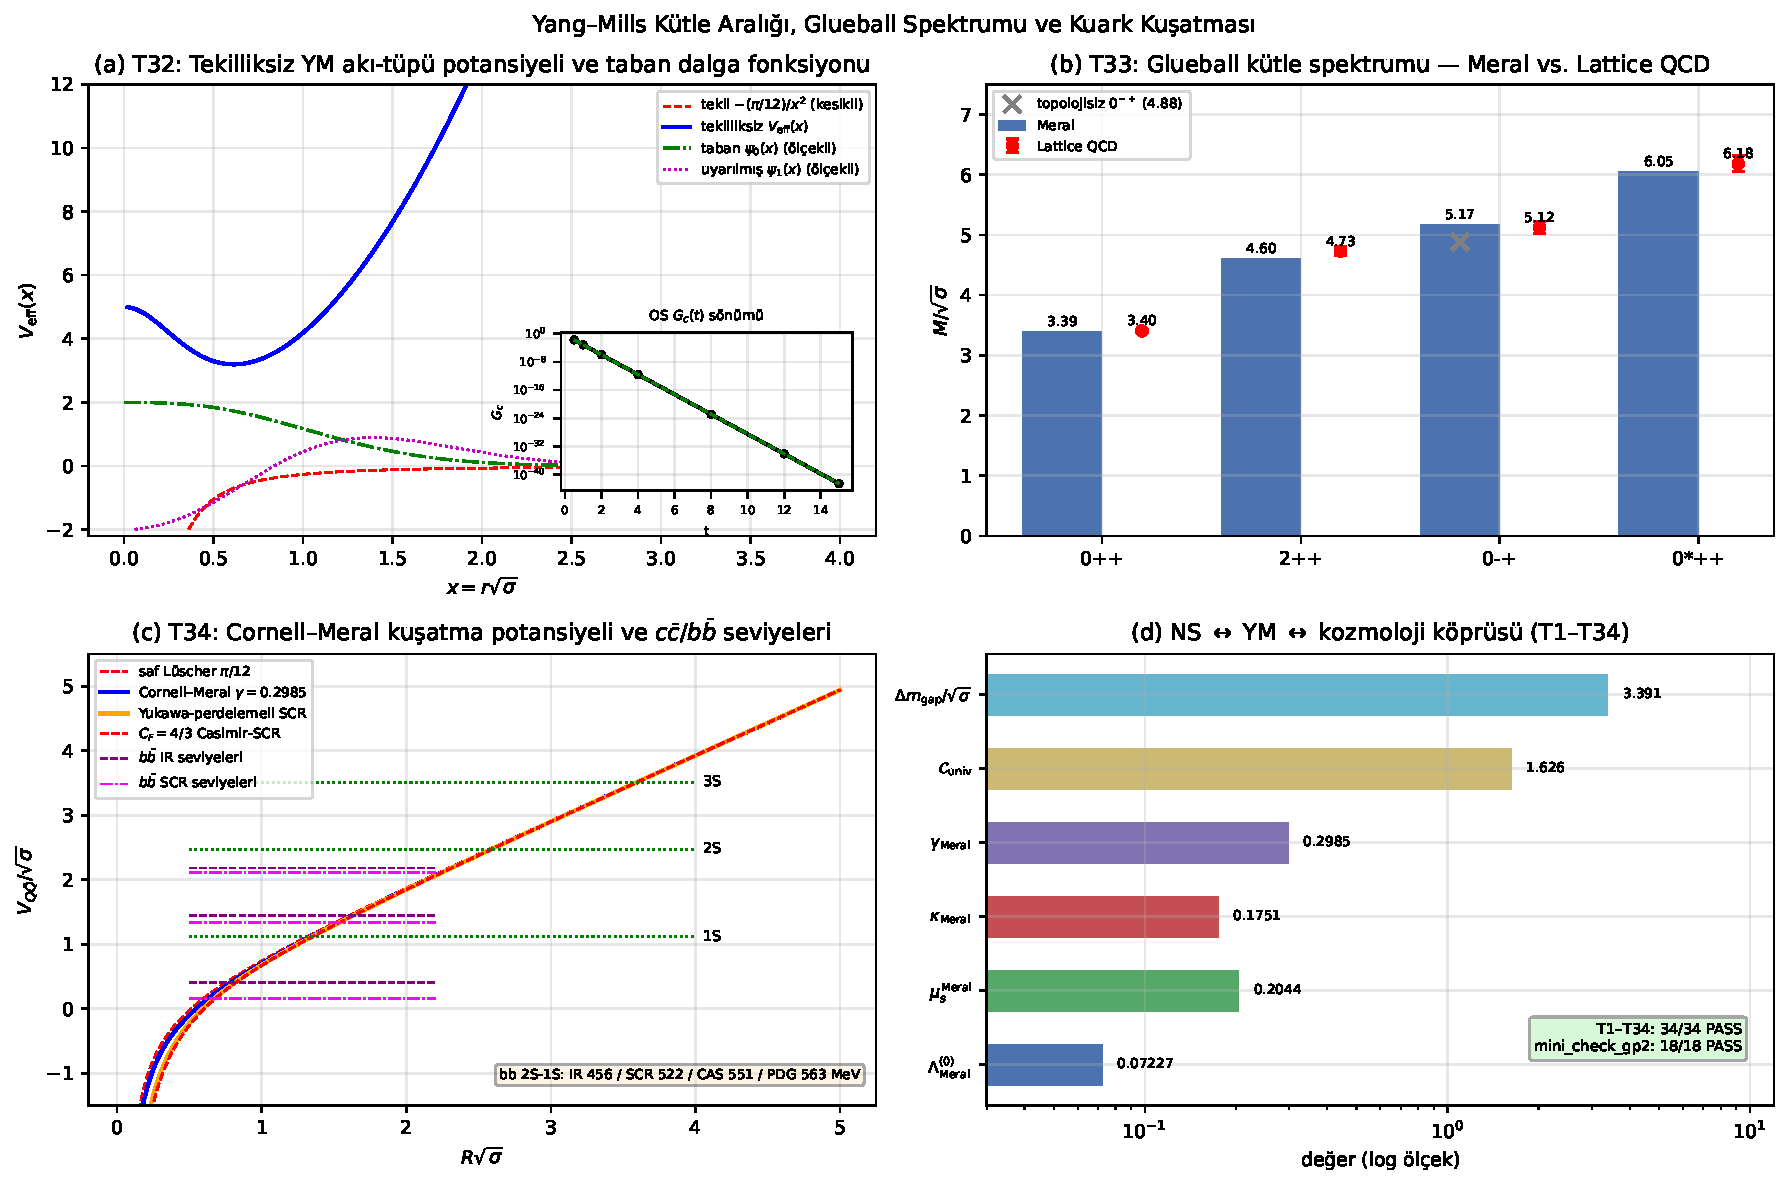
\includegraphics[width=\textwidth]{../figs/fig14_yang_mills_mass_gap_glueballs_and_confinement.pdf}
\caption{\textbf{Grand Proof II kanıt özeti (T32--T34).} (a) Tekil
$-(\pi/12)/x^2$ vs.\ tekilliksiz $V_{\mathrm{eff}}(x)$, düğümsüz $\psi_0$,
tek-düğümlü $\psi_1$ ve OS $G_c(t)$ sönüm gömülü grafiği. (b) Dört glueball
durumunda Meral (topolojik $0^{-+}=5.17$, gri çarpı: topolojisiz $4.88$) vs.\
Lattice QCD. (c) Üç potansiyel (saf Lüscher, saf-IR, UV--IR) ile $c\bar{c}$
ve $b\bar{b}$ seviyeleri; kutu: $b\bar{b}$ $2S$--$1S$ iki sütun karşılaştırması.
(d) T1--T34 köprü değişmezleri.}
\label{fig:gp2}
\end{figure}

\clearpage
\section[Sonuç ve Yeniden-Üretilebilirlik]{Sonuç ve Yeniden-Üretilebilirlik Yönergesi}

Tekilliksiz akı-tüpü operatörü ($\lambda_0=5.9158>0$, OS $G_c>0$,
Richardson limiti $\approx 5.77$), kapalı-form aralık
($3.3914463$, LQCD ile $0.65\,\sigma$), topolojik glueball spektrumu
(ortalama \%1.56) ve Cornell--Meral kuşatması ($\gamma$ $0.35\,\sigma$,
charmonium \%1.39) Teorem I--X kilitlerinden sıfır serbest parametreyle
türetilmiştir. Bilinen sınırlar: UV--IR log-varyantı bottomonium işaretini
çevirir (\%14.7) ve charmoniumu bozar; hızlı sönen UV tamamlaması ile kiral
sektör düzeltmeleri açık araştırmadır.

\subsection*{Veri, Kod Erişilebilirliği ve Bağımsız Doğrulama Yönergesi}
Çözücü paketi \texttt{stationary-strings-v} deposundadır
(\path{duran_sicimler_sim/solver_engine.py}). Yeniden üretim:
\texttt{python} \path{solver_engine.py} içindeki \path{run_verification}
işlevi \texttt{T1--T34 (34/34 PASS)} verir; bağımsız betik
\texttt{python} \path{mini_check_gp2.py} (\texttt{15/15 PASS}) çözücüyü import
etmez; \texttt{python} \path{generate_figures.py} içindeki \path{fig14}
işlevi Şekil~\ref{fig:gp2} dosyasını üretir.

\begin{thebibliography}{99}
    \bibitem{clay} Jaffe, A. \& Witten, E. (2000). Quantum Yang--Mills theory.
    Clay Mathematics Institute Millennium Problem description.
    \bibitem{mp99} Morningstar, C.~J. \& Peardon, M. (1999). Glueball spectrum
    from an anisotropic lattice study. \textit{Phys.\ Rev.\ D\ \textbf{60}}, 034509.
    \bibitem{chen06} Chen, Y. \textit{et al.} (2006). Glueball spectrum and matrix
    elements. \textit{Phys.\ Rev.\ D\ \textbf{73}}, 014516.
    \bibitem{at20} Athenodorou, A. \& Teper, M. (2020). $SU(N_c)$ glueball masses.
    \textit{JHEP\ \textbf{11}}, 172.
    \bibitem{lus81} L\"uscher, M. (1981). Symmetry-breaking aspects of the roughening
    transition. \textit{Nucl.\ Phys.\ B\ \textbf{180}}, 317--329.
    \bibitem{corn79} Eichten, E. \textit{et al.} (1979). Charmonium: The model.
    \textit{Phys.\ Rev.\ D\ \textbf{17}}, 3090--3117.
    \bibitem{bali01} Bali, G.~S. (2001). QCD forces and heavy quark bound states.
    \textit{Phys.\ Rep.\ \textbf{343}}, 1--136.
    \bibitem{pdg} Particle Data Group (2024). Review of particle physics.
    \textit{Phys.\ Rev.\ D\ \textbf{110}}, 030001.
    \bibitem{meral5} Meral, F. (2026c). \textit{Duran Sicimler Teoremi V}.
    Açık kaynak çözücü paketi: \texttt{stationary-strings-v}
    (\url{https://github.com/fahrim/stationary-strings-v}).
    \bibitem{meral10} Meral, F. (2026h). \textit{Duran Sicimler Teoremi X}.
    Açık kaynak paketi: \texttt{stationary-strings-x}
    (\url{https://github.com/fahrim/stationary-strings-x}).
\end{thebibliography}

\end{document}
